\documentclass[conference]{../../LaTex_Template/IEEEtran}
\IEEEoverridecommandlockouts
\usepackage{cite}
\usepackage{xeCJK}
\setCJKmainfont{Songti SC}
\usepackage{amsmath,amssymb,amsfonts}
\usepackage{graphicx}
\usepackage{textcomp}
\usepackage{float}
\graphicspath{{../../../results/figures/}{../figures/}}

\begin{document}

\title{具有需求学习与参考价格效应的动态定价：复现实验与稳健校准扩展}

\author{
\IEEEauthorblockN{罗靖炆}
\IEEEauthorblockA{学号：72542176\\
SDSC8008 Data-driven Operations Research}
}

\maketitle

\begin{abstract}
本报告研究 den Boer 与 Keskin 关于“具有需求学习与参考价格效应的动态定价”的模型、理论逻辑和数值实验。报告目标有三点：第一，解释参考价格效应为什么会让动态定价不同于普通 learning-and-earning 问题；第二，复现论文主要数值证据；第三，基于运筹学中的稳健设计思想，加入一个关于 slow-moving policy 参数校准的新扩展实验。为保持表述严谨，本文将已发表研究中转储后的数值结果称为 Published Study Benchmark (PSB)，将本项目重新生成的独立仿真实验称为 Independent Replication Experiment (IRE)，下文均使用 PSB 和 IRE 简称。IRE 复现了论文的核心结论：deterministic testing 在无参考效应环境下表现良好，但在 reference-effect 场景下 regret 明显增大；slow-moving pricing 通过同时管理需求估计与参考价格状态，使 regret 保持较低水平。新增的 Reference-Aware Robust Calibration (RARC) 实验进一步显示，在参考价格记忆和损失侧参考效应不确定时，更小的初始扰动和更慢的扰动衰减可以改善最坏情形 regret。
\end{abstract}

\section{背景、动机与核心思想}
动态定价是数据驱动运筹学中的经典问题。卖家需要反复选择价格、观察需求、更新需求曲线估计，并最大化长期累计收入。即使在没有行为效应的普通模型中，问题也存在探索与收益的权衡：价格变化可以帮助估计需求，但不合适的探索价格会降低当期收入。已有研究大量讨论未知需求参数下的在线定价学习问题 \cite{broderRusmevichientong2012,keskinZeevi2014}。

目标论文在这一框架中加入了一个重要行为状态变量：参考价格。消费者通常不会只根据当前价格本身作出购买决策，而是会把当前价格与记忆中或预期中的参考价格比较。如果当前价格低于参考价格，消费者可能感到获得；如果当前价格高于参考价格，消费者可能感到损失。这一思想与参考依赖偏好和损失厌恶有关 \cite{tverskyKahneman1991}，也常用于解释促销、折扣和价格上涨对后续购买行为的影响 \cite{popescuWu2007}。

该问题的运筹学难点在于参考价格是内生状态。它由历史价格形成，又会反过来影响未来需求。因此，一次价格试探具有双重作用：一方面提供需求学习数据，另一方面改变未来需求所依赖的参考价格状态。价格不是被动观测工具，而是改变系统状态的干预变量。如果卖家仍使用无参考效应模型下的普通学习策略，就可能把参考价格造成的需求变化误认为需求截距或斜率变化，导致估计最优价长期偏离正确水平。

den Boer 与 Keskin 的核心思想是：需求学习和参考价格控制必须联合设计。价格变化既要提供统计信息，也要避免过度扰动参考价格状态。slow-moving pricing 通过越来越长的 episode 和逐渐缩小的双侧扰动实现这一思想。在每个 episode 内，价格变化足够缓慢，使参考价格逐渐靠近当前价格区域，从而降低不可观测状态对需求估计的污染。

本报告的复现实验围绕两类策略展开。第一类是 deterministic testing，它定期发布两个固定测试价，其余时期发布估计最优价，是无参考效应动态定价中自然的 learning-and-earning 策略。第二类是 slow-moving pricing，它显式控制价格变化节奏。两者对比能够回答本文最核心的问题：在存在参考价格效应的市场中，策略结构是否比单纯收集更多需求数据更重要。

Figure~\ref{fig:referencefeedback} 概括了参考价格反馈机制。同一个价格决策会同时进入当前需求、当前收入、未来参考价格更新和下一轮学习过程。因此，探索不能只被理解为数据收集，也必须被理解为会改变系统状态的干预。

\begin{figure*}[!t]
  \centering
  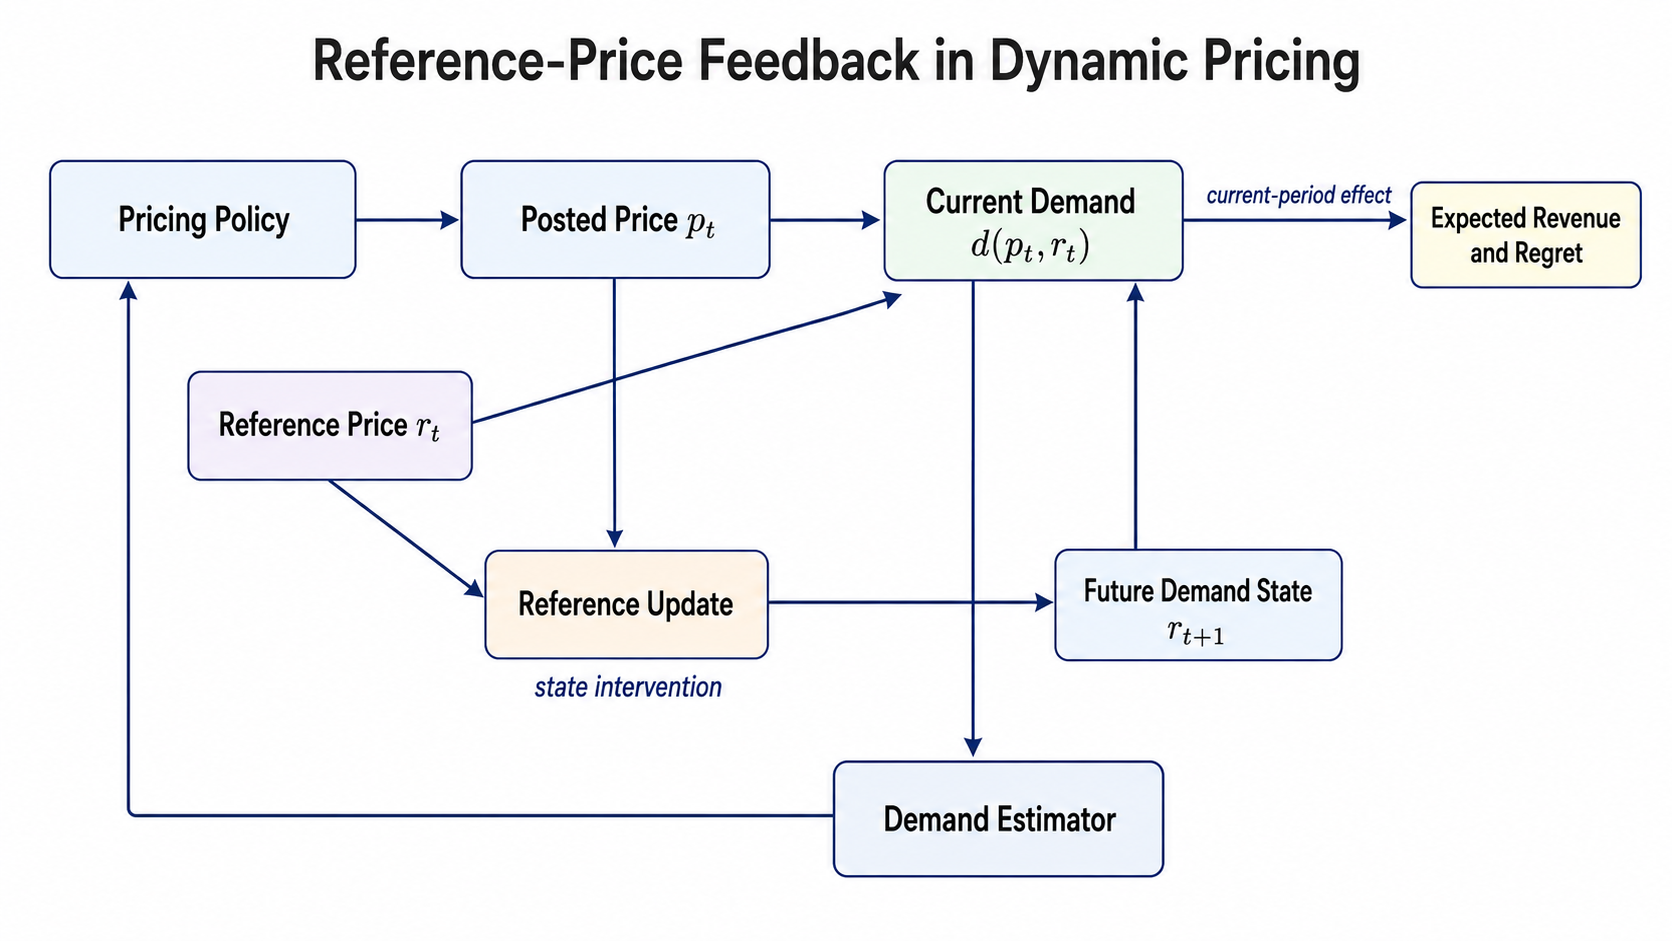
\includegraphics[width=0.92\textwidth]{reference_feedback.png}
  \caption{参考价格反馈机制。价格行为既影响当前需求，也改变后续需求观测所依赖的参考价格状态。}
  \label{fig:referencefeedback}
\end{figure*}

\section{模型、理论与应用}
\subsection{需求模型}
复现使用的需求模型为
\begin{equation}
d_t = \alpha - \beta p_t + \eta^+(r_t-p_t)^+ - \eta^-(p_t-r_t)^+ + \epsilon_t,
\label{eq:demand}
\end{equation}
其中 $p_t$ 是当前价格，$r_t$ 是参考价格，$\epsilon_t$ 是零均值需求冲击。IRE 采用 $\beta>0$ 的正号价格敏感度记法，因此直接价格效应为 $-\beta p_t$。当价格低于参考价时，$\eta^+(r_t-p_t)^+$ 表示获得感带来的需求提升；当价格高于参考价时，$-\eta^-(p_t-r_t)^+$ 表示损失感带来的需求下降。主实验中 $\eta^+=0.1$、$\eta^-=0.3$，体现损失效应强于获得效应。

参考价格采用指数平滑更新：
\begin{equation}
r_{t+1} = \zeta r_t + (1-\zeta)p_t,\quad \zeta \in [0,1).
\label{eq:reference}
\end{equation}
$\zeta$ 越小，参考价格对当前价格反应越快；$\zeta$ 越大，参考价格记忆越长。主复现实验使用 $\zeta=0.1$。新增 RARC 扩展会改变 $\zeta$，因为参考价格记忆长度是实际定价场景中很难精确知道的关键参数。

给定参数 $\theta=(\alpha,\beta,\eta^+,\eta^-)$，单期期望收入为
\begin{equation}
R(p,r,\theta)=p\left[\alpha-\beta p+\eta^+(r-p)^+-\eta^-(p-r)^+\right].
\end{equation}
当参考效应为零或被忽略时，静态最优价格为 $\alpha/(2\beta)$，并限制在可行价格区间内。默认参数 $\alpha=1.1$、$\beta=0.5$ 对应 $p^\star=1.1$。

\subsection{Regret 与理论逻辑}
论文使用累计 regret 衡量策略性能：
\begin{equation}
\Delta_\pi(T,\rho,\theta)=\Pi^\star(T,\rho,\theta)
-\mathbb{E}_\pi\left[\sum_{t=1}^T R(p_t,r_t,\theta)\right].
\end{equation}
其中 benchmark 是知道真实需求参数与参考价格过程的全信息决策者。精确动态 benchmark 的形式并不简单，但论文证明，在 loss-averse 的时变参考价格场景下，固定价格 $p^\star=\alpha/(2\beta)$ 是有用的比较基准。若卖家持续发布同一价格，参考价格会以几何速度靠近该价格，因此由参考价格偏离造成的累计损失可以被控制。

理论机制可以概括为三步。第一，稳定价格路径可以避免参考价格状态过度漂移。第二，如果策略在越来越长的阶段内保持价格相对稳定，需求观测中的状态污染会变小。第三，逐渐缩小的双侧扰动仍能提供足够的价格变化用于估计需求。slow-moving pricing 正是利用这三点，在未知需求和参考价格效应同时存在时达到 $O(\sqrt{T})$ regret，与该类未知需求定价问题的基本下界同阶。

\subsection{应用含义}
该模型适用于重复零售定价、订阅续费定价、在线平台价格实验和促销日历等场景。在这些场景中，消费者会从历史价格中形成“正常价格”或“公平价格”的预期。频繁打折可能降低消费者参考价格，突然涨价可能带来强烈损失感。因此，企业不应只用短期销量评价价格实验，也应评估实验如何改变未来消费者预期。

从运筹学角度看，slow-moving pricing 是一种有纪律的实验设计。它不是完全避免探索，而是用局部、缓慢、可解释的价格扰动来探索。它的 episode 结构控制潜在状态，双侧扰动提供估计信息。这使策略不仅有理论意义，也更容易被解释为实际业务中的稳健价格测试方案。

\section{IRE 设计与命名}
\subsection{PSB 与 IRE}
本文使用两类数值来源。Published Study Benchmark (PSB) 指已发表研究中释放的数值结果在转储后的结构化数据；Independent Replication Experiment (IRE) 指本项目根据需求函数和参考价格更新公式重新生成的仿真实验。PSB 只作为对比和可视化来源，IRE 使用确定性随机种子生成新的仿真路径。

这个区分很重要。IRE 不追求与 PSB 每条路径逐点相同，因为两者随机流并不匹配。更合理的判断标准是：策略排序、曲线形态、最终数量级和机制解释是否一致。因此，Figure 2--5 均采用三视图布局：PSB 单独图、IRE 单独图，以及同坐标系叠加图。

\subsection{流程与参数}
实验流程分三步。第一，将已发表研究中的数值输出转储为 `data/processed/' 下的 `.npz' 和 CSV 文件。第二，运行 deterministic testing 与 slow-moving pricing 的 IRE 仿真。第三，生成 Figure 2--5 对比图和汇总表。

Figure~\ref{fig:pipelineworkflow} 展示了本项目的复现实验管线。PSB 分支提供转储后的基准曲线，IRE 分支从 Python 模型模块重新生成仿真曲线；二者只在可视化比较和汇总表阶段合并。

\begin{figure*}[!t]
  \centering
  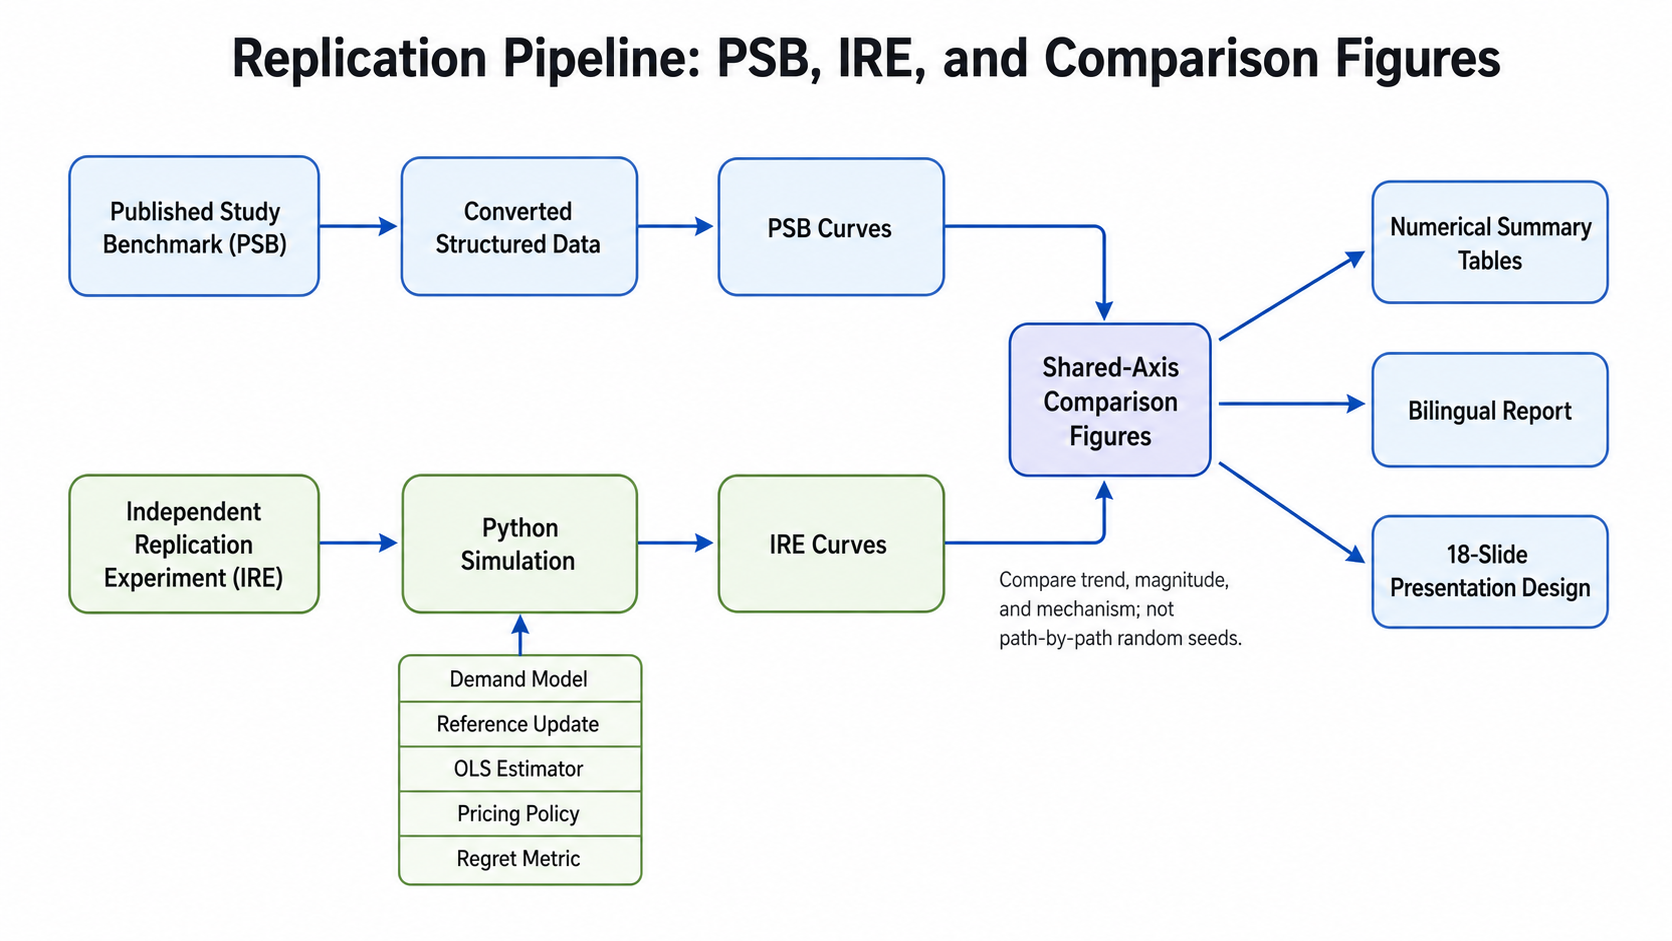
\includegraphics[width=0.92\textwidth]{replication_pipeline.png}
  \caption{复现实验管线。PSB 与 IRE 在生成同坐标系对比图和数值汇总前保持分离。}
  \label{fig:pipelineworkflow}
\end{figure*}

主实验参数为 $\alpha=1.1$、$\beta=0.5$、$\sigma=0.1$、$\zeta=0.1$，时间长度 $T=10000$，仿真路径数为 10，价格区间为 $[0.5,1.5]$。实验包含两种需求环境：无参考效应环境设置 $\eta^+=\eta^-=0$；reference-effect 环境设置 $\eta^+=0.1$、$\eta^-=0.3$。regret 使用期望收入计算，实现需求只用于估计器更新，因此随机噪声不会混入理论收入比较。

\subsection{策略实现}
deterministic testing 使用价格区间三分点和三分之二点作为固定测试价。在默认价格区间下，这两个测试价约为 $0.8333$ 和 $1.1667$。非测试期中，策略用线性最小二乘估计需求参数，并发布截断后的 plug-in 价格：
\begin{equation}
\hat p_t^\star = \frac{\hat\alpha_t}{2\hat\beta_t}.
\end{equation}
该策略在无参考效应模型下自然且有效，但它没有管理参考价格状态。

slow-moving pricing 采用 episode 结构。第 $i$ 个 episode 中，策略围绕当前估计最优价做双侧扰动 $\delta_i$。半段长度满足 $n_i=2^i$，主复现实验中的扰动幅度满足 $\delta_i=c_0 2^{-i/4}$。每个 episode 结束后，策略更新需求估计和估计最优价。越来越长的 episode 使参考价格靠近当前价格区域，双侧扰动则保留局部估计所需的信息。

\section{复现实验结果}
\subsection{最终数值汇总}
Table~\ref{tab:comparison} 给出最终时期的 PSB/IRE 对比。IRE 复现了 PSB 的主要策略排序：deterministic testing 在无参考效应下 regret 很低，但在 reference-effect 场景下 regret 大幅上升；slow-moving pricing 在两种环境下都保持低 regret。

\begin{table*}[t]
\centering
\caption{最终时期 PSB 与 IRE 结果对比。}
\label{tab:comparison}
\begin{tabular}{llllrrr}
\hline
图 & 策略 & 场景 & 指标 & PSB & IRE & 相对差异\\
\hline
2 & Deterministic testing & 无参考效应 & 最终平均 regret & 12.18 & 9.67 & -20.63\%\\
2 & Deterministic testing & 有参考效应 & 最终平均 regret & 328.79 & 299.51 & -8.90\%\\
3 & Deterministic testing & 无参考效应 & 最终平均估计价格 & 1.095 & 1.090 & -0.45\%\\
3 & Deterministic testing & 有参考效应 & 最终平均估计价格 & 0.850 & 0.860 & 1.24\%\\
4 & Slow-moving & 有参考效应 & 最终平均参考价格 & 1.097 & 1.076 & -1.90\%\\
4 & Slow-moving & 有参考效应 & 最终平均估计价格 & 1.109 & 1.088 & -1.88\%\\
5 & Slow-moving & 无参考效应 & 最终平均 regret & 7.61 & 11.86 & 55.88\%\\
5 & Slow-moving & 有参考效应 & 最终平均 regret & 10.40 & 12.33 & 18.59\%\\
\hline
\end{tabular}
\end{table*}

\subsection{Deterministic Testing}
Figure~\ref{fig:figure2} 展示 deterministic testing 的 regret。无参考效应时，PSB 与 IRE 曲线都保持低水平，最终平均 regret 分别为 $12.18$ 和 $9.67$。相对于 $10000$ 的时间长度，这说明该策略在模型正确时能够有效学习。

reference-effect 场景则完全不同。最终平均 regret 上升到 $328.79$ 和 $299.51$。叠加图显示两条曲线具有一致的定性形态：引入参考效应后，regret 增长速度明显加快。策略仍然在收集数据，但这些数据已经被不可观测参考价格状态污染。

\begin{figure*}[t]
  \centering
  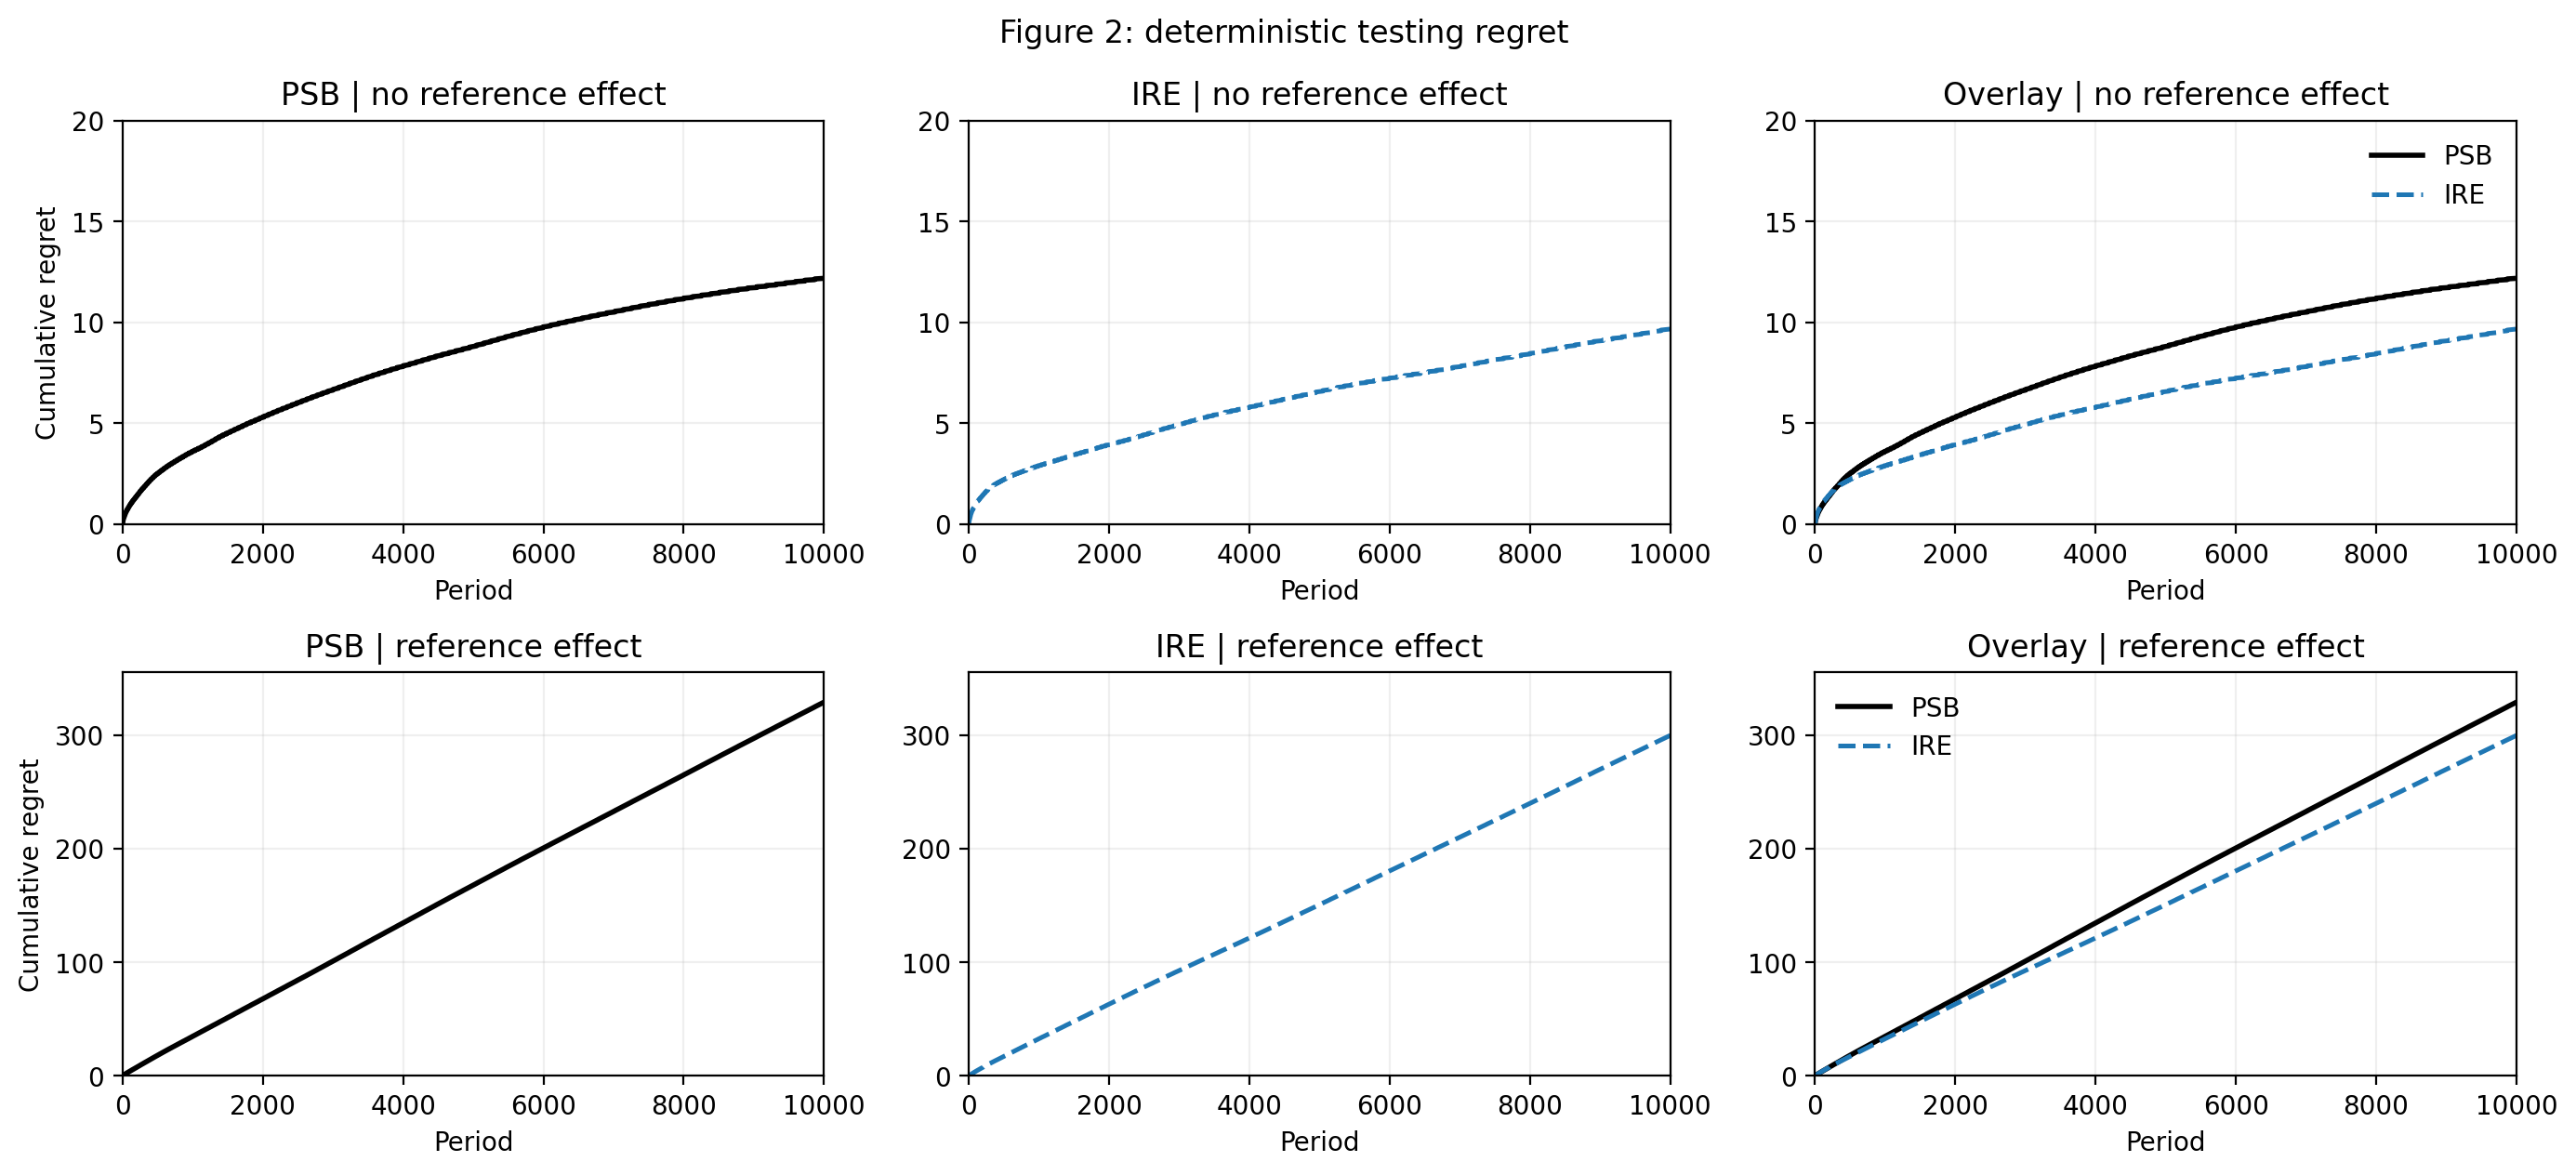
\includegraphics[width=0.96\textwidth]{figure2_comparison.png}
  \caption{Figure 2 对比。每行对应一个环境；三列分别展示 PSB、IRE 与同坐标叠加视图。}
  \label{fig:figure2}
\end{figure*}

Figure~\ref{fig:figure3} 解释了失败机制。无参考效应时，估计价格逐渐靠近 $p^\star=1.1$。有参考效应时，最终平均估计价格稳定在 $0.85$--$0.86$ 附近，明显低于 benchmark。这不是最小二乘的数值失败，而是模型失配。真实需求同时取决于当前价格和参考价格状态，但回归模型主要把价格作为解释变量；参考状态又由历史价格生成，因此其影响会被错误写入估计截距和斜率。

\begin{figure*}[t]
  \centering
  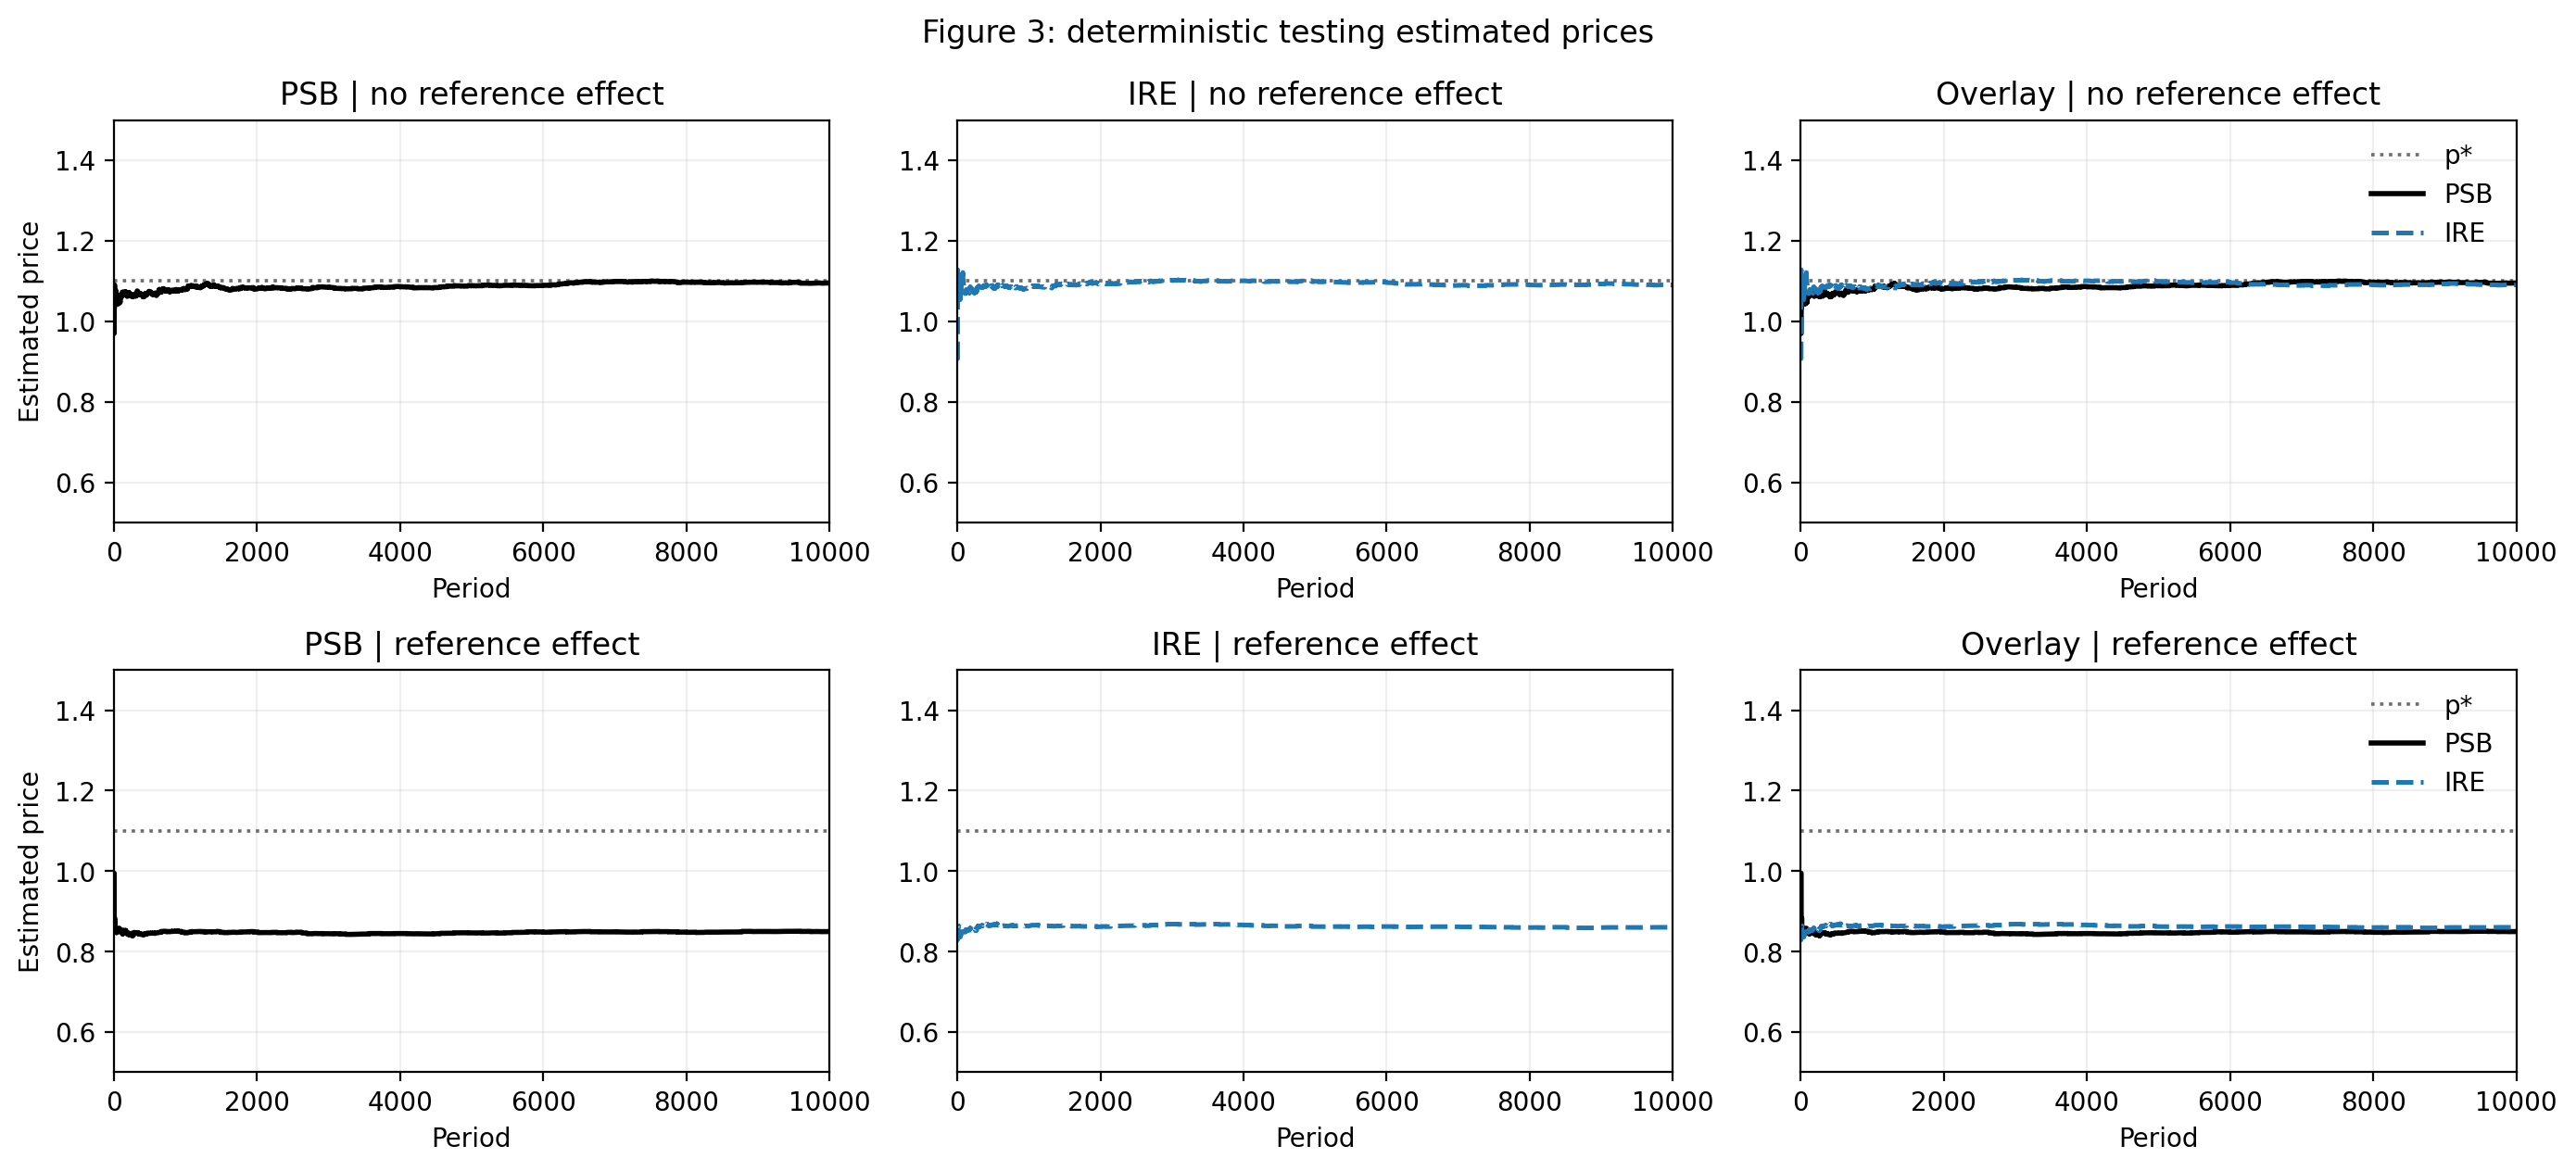
\includegraphics[width=0.96\textwidth]{figure3_comparison.png}
  \caption{Figure 3 对比。reference-effect 场景下 deterministic testing 的估计价格稳定在 benchmark 下方。}
  \label{fig:figure3}
\end{figure*}

\subsection{Slow-Moving Pricing}
Figure~\ref{fig:figure4} 展示 reference-effect 场景下 slow-moving pricing 的参考价格和估计价格路径。最终平均参考价格为 $1.097$ 与 $1.076$，最终平均估计价格为 $1.109$ 与 $1.088$。与 Figure~\ref{fig:figure3} 中的偏差相比，这些结果更接近 $p^\star=1.1$。

\begin{figure*}[t]
  \centering
  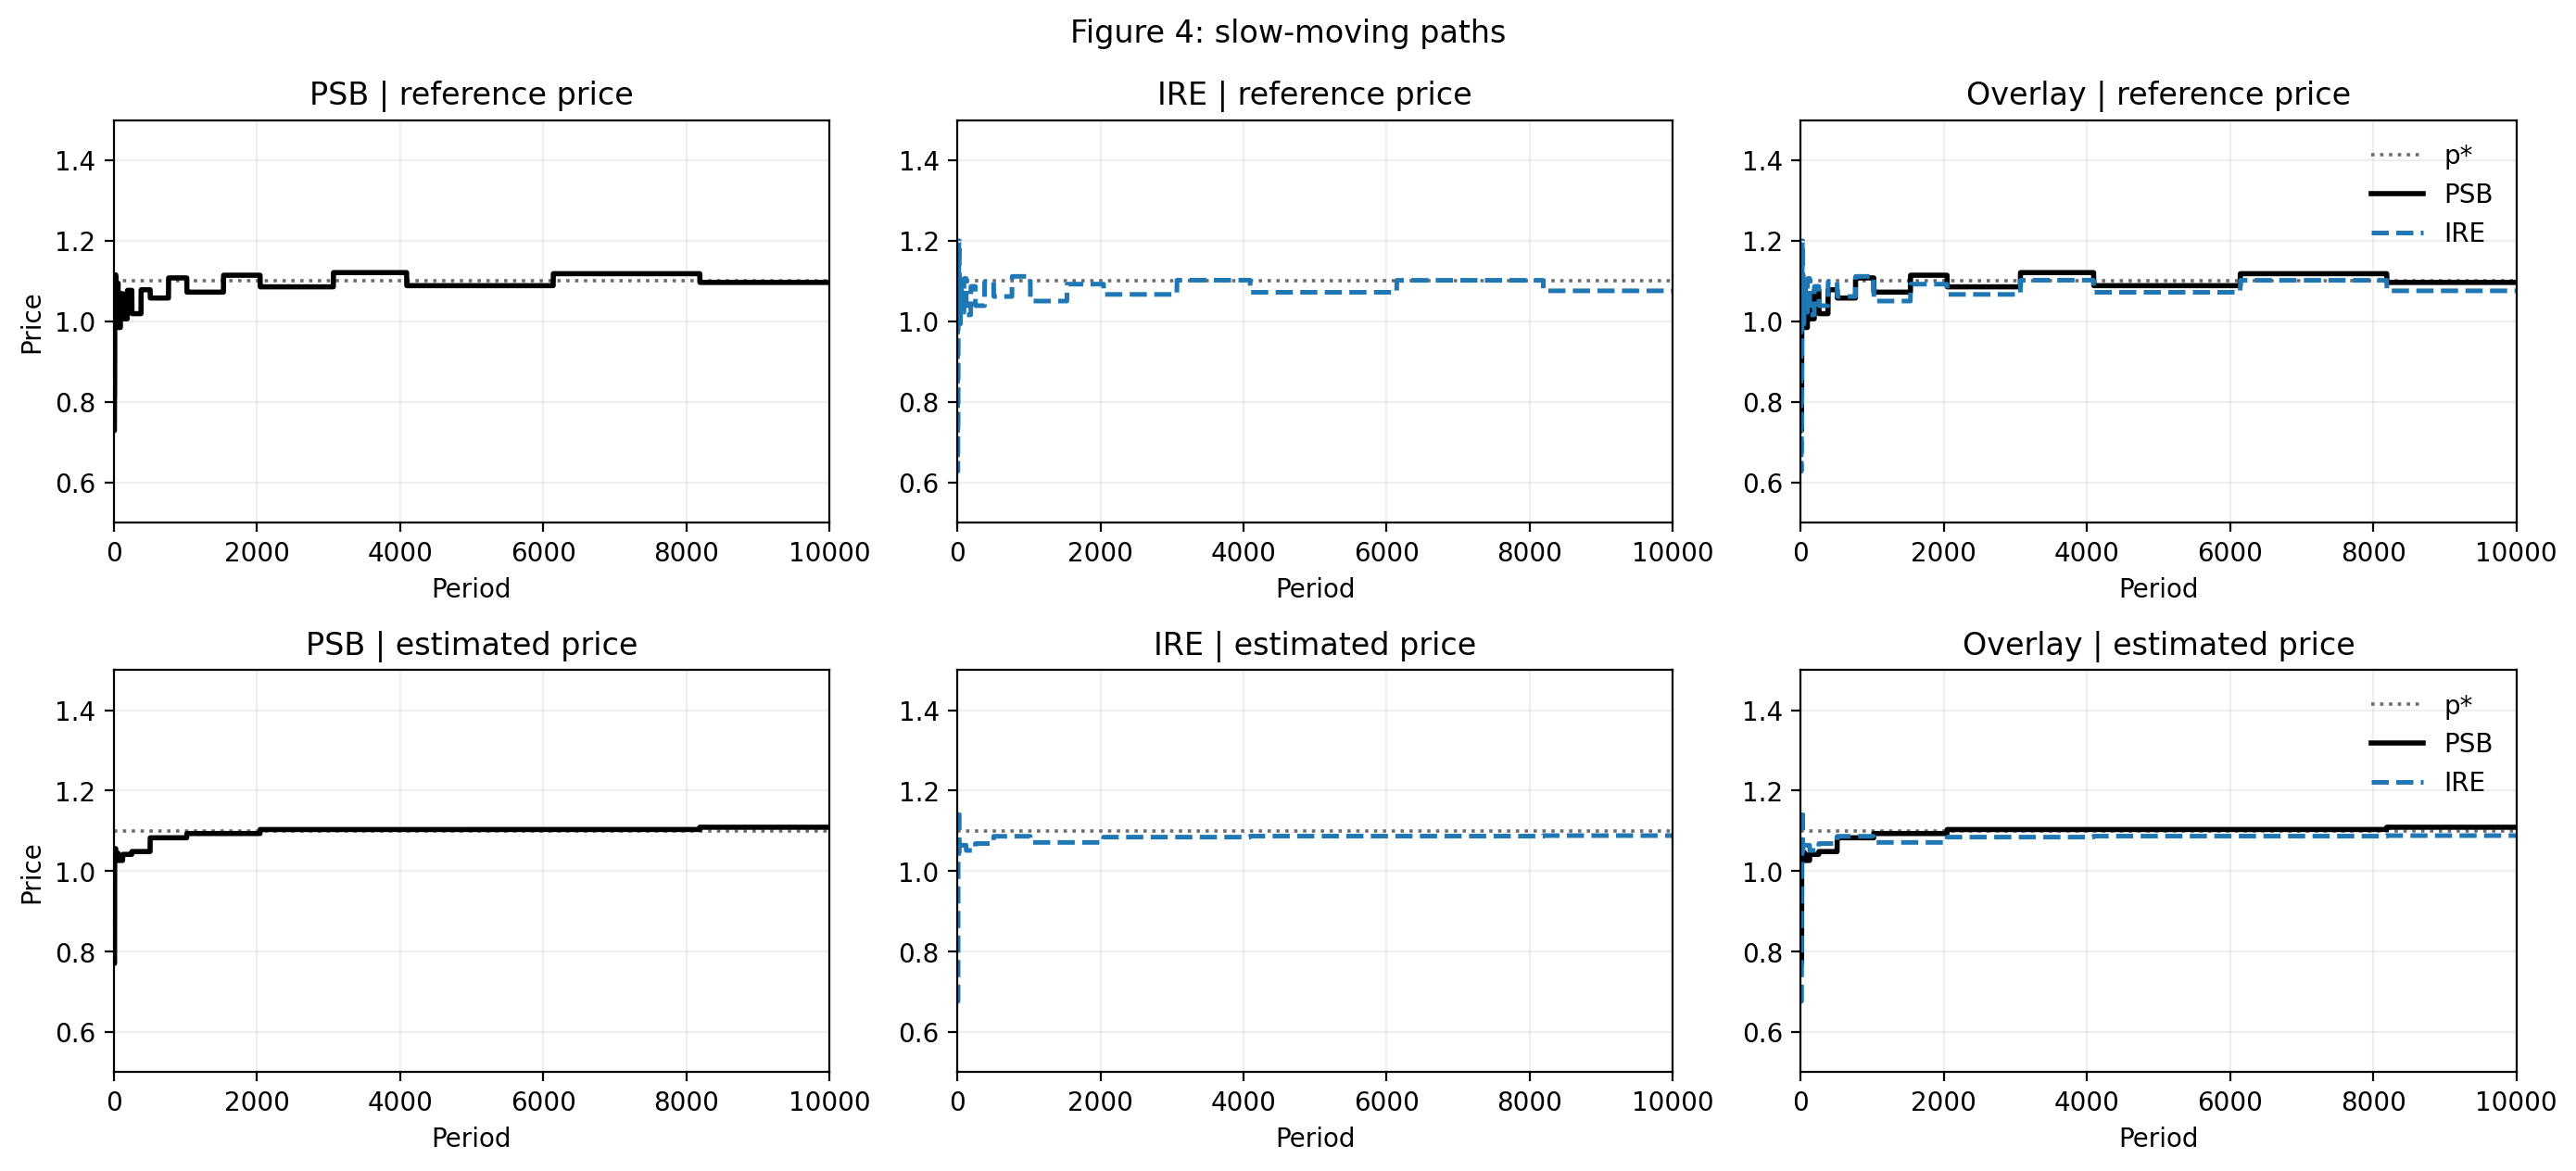
\includegraphics[width=0.96\textwidth]{figure4_comparison.png}
  \caption{Figure 4 对比。slow-moving pricing 使参考价格和估计价格保持在 benchmark 附近。}
  \label{fig:figure4}
\end{figure*}

Figure~\ref{fig:figure5} 展示 slow-moving pricing 的 regret。IRE 的最终 regret 在无参考效应和有参考效应场景下分别为 $11.86$ 和 $12.33$；PSB 对应值为 $7.61$ 和 $10.40$。具体数值不同，但两种环境都保持在低 regret 量级。相比之下，deterministic testing 在加入参考效应后从约 $10$ 上升到约 $300$。

\begin{figure*}[t]
  \centering
  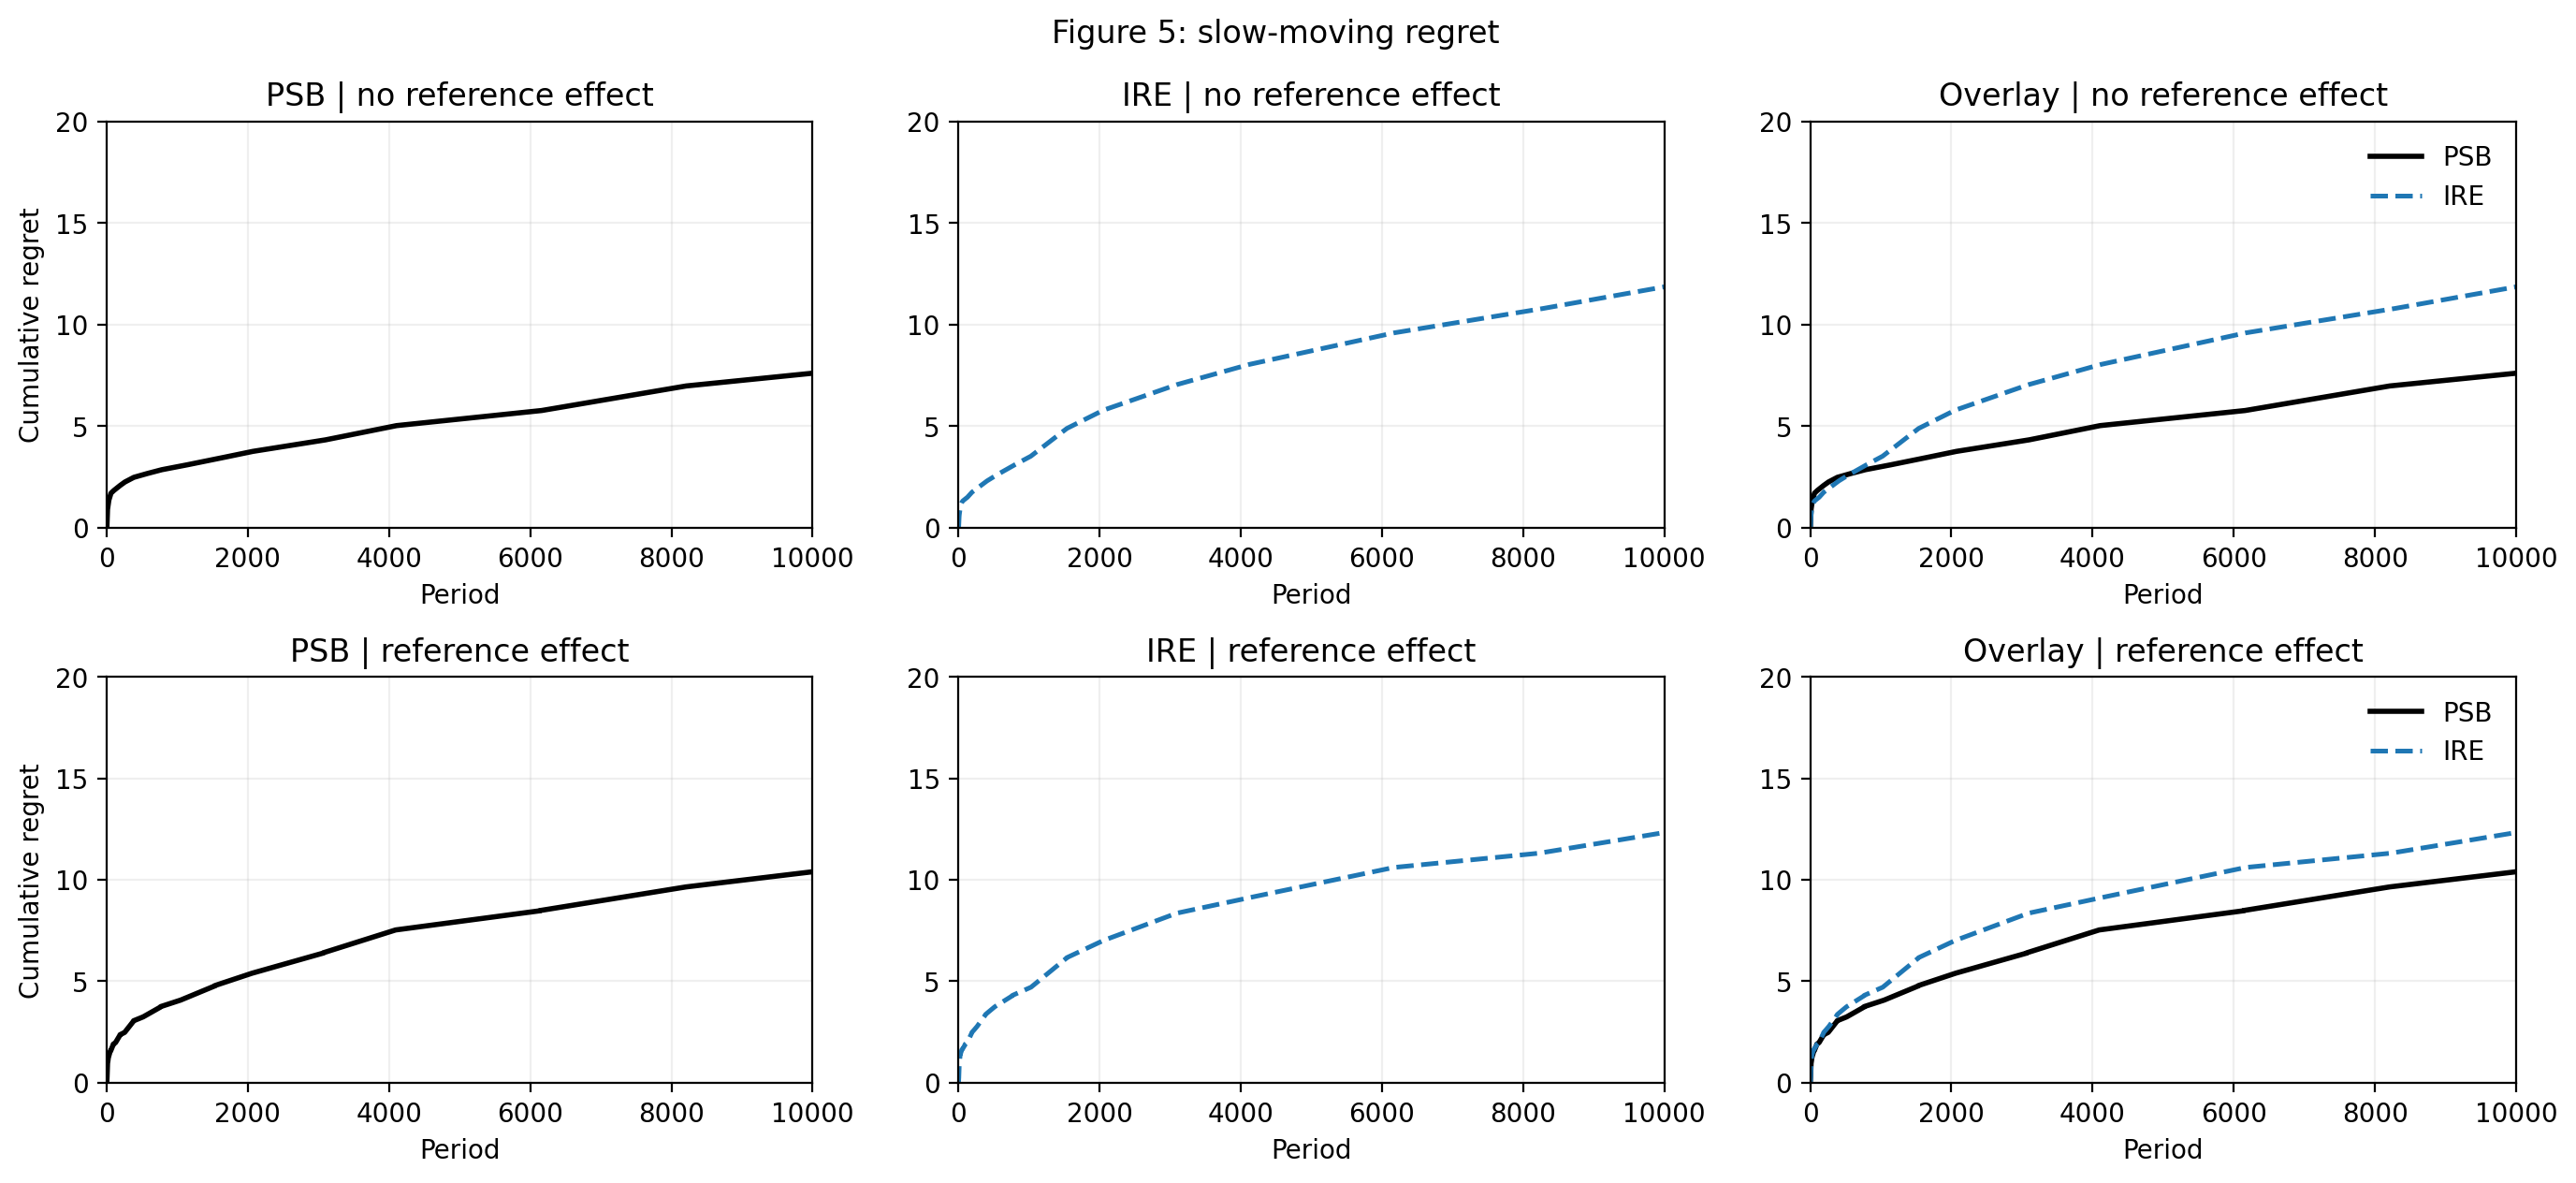
\includegraphics[width=0.96\textwidth]{figure5_comparison.png}
  \caption{Figure 5 对比。slow-moving pricing 在无参考效应和有参考效应环境下都保持较低 regret。}
  \label{fig:figure5}
\end{figure*}

\section{机制层面分析}
复现实验的关键不是某个点的数值完全相同，而是两类探索逻辑的差异。deterministic testing 把探索视为外生信息收集：在预定时期发布测试价，估计需求曲线，然后利用估计值定价。这一逻辑在需求只取决于当前价格时成立。但在存在参考效应时，测试价本身会改变未来参考价格，下一期需求观测也会受到当前试探的影响。

slow-moving pricing 改变了学习环境。通过较长 episode，它让参考价格有时间靠近当前价格区域；通过逐渐缩小扰动，它减少探索价格与估计最优价之间的差距。这样并没有消除参考价格效应，但使状态变化更可控，需求观测更接近普通估计器能够处理的局部环境。换言之，slow-moving pricing 将一个被状态污染的学习问题，转化为更稳定的局部学习问题。

这也解释了为什么 PSB/IRE 比较应关注策略层面的趋势而非逐点一致。十条仿真路径下，随机流差异会影响具体数值。但更重要的证据是同一结构性对比在两组结果中同时出现：deterministic testing 在无参考效应下稳健，在 reference-effect 场景下脆弱；slow-moving pricing 在两种场景下都稳定。

Figure~\ref{fig:policymechanism} 将这一机制差异可视化。deterministic testing 产生较大的价格跳动，并在参考状态已经被扰动的需求观测上估计参数；slow-moving pricing 则用局部扰动和更长 episode 降低这种状态污染。

\begin{figure*}[!t]
  \centering
  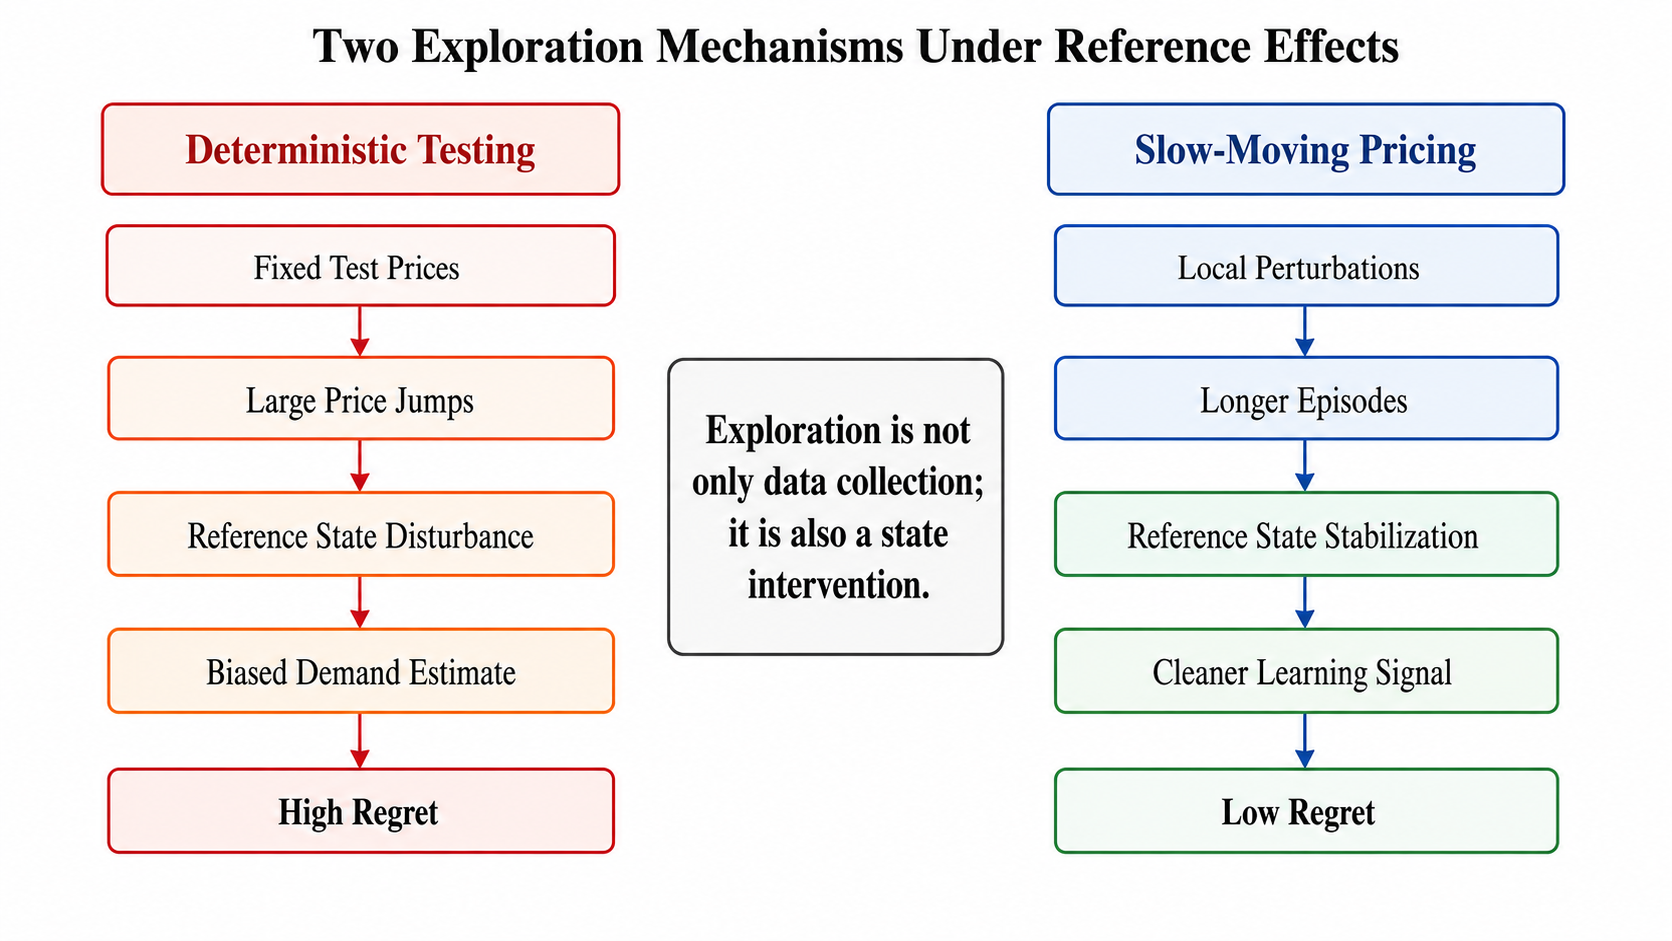
\includegraphics[width=0.92\textwidth]{exploration_mechanisms.png}
  \caption{探索机制对比。deterministic testing 将探索视为数据收集，而 slow-moving pricing 将探索视为会改变状态的干预。}
  \label{fig:policymechanism}
\end{figure*}

\begin{table*}[t]
\centering
\caption{数值证据与运筹学机制的对应关系。}
\label{tab:evidence}
\resizebox{\textwidth}{!}{%
\begin{tabular}{llll}
\hline
证据 & 主要观察 & 支持的机制 & 运营含义\\
\hline
Figure 2 无参考效应 & deterministic testing regret 较低 & 无状态污染时普通学习有效 & 记忆弱市场可使用标准价格试探\\
Figure 2 有参考效应 & regret 上升到约 300 & 测试价改变参考状态 & 探索会损伤未来需求环境\\
Figure 3 & 估计价格稳定在约 0.85 & 状态效应污染需求估计 & 有偏 plug-in 价格可能看似稳定\\
Figure 4 & 参考价与估计价接近 1.1 & 慢变化降低状态污染 & 渐进式测试提升观测可靠性\\
Figure 5 & slow-moving regret 保持低量级 & 学习和状态控制相互配合 & 状态感知探索避免长期损失\\
RARC & 小扰动候选最稳健 & 参数校准影响稳健性 & 定价实验需考虑行为记忆风险\\
\hline
\end{tabular}
}
\end{table*}

\section{复现控制与实现可靠性}
本项目的实现遵循三个复现原则。第一，PSB 数据先转储，再用于比较；IRE 仿真不直接读取源数据。这样可以将比较数据、仿真代码和图表生成过程分开检查，保证每一步都是可追踪的。

第二，实现需求与期望收入严格分离。实现需求包含随机冲击，用于更新估计器；regret 使用期望收入计算，符合理论定义。若把随机需求直接混入 regret，就会把策略损失和随机噪声混在一起，降低曲线解释性。

第三，IRE 使用确定性随机种子。虽然不追求逐点匹配 PSB，但同一命令可以重复生成相同 IRE 结果。这样后续若增加新策略或扩展实验，结果变化可以归因于策略本身，而不是随机样本变化。

代码结构也对应论文数学结构。需求函数、参考价格更新、最小二乘估计器、定价策略、regret 度量、数据转储和绘图被分离到不同模块。这样做不仅是软件工程上的清晰，也能减少概念混淆。例如，参考价格更新属于环境状态变化，不能被误写成普通估计器内部逻辑；理论 regret 使用期望收入，也不能被实现需求替代。

验证分为两层。单元测试检查需求函数左右分段、指数平滑参考价格、静态最优价格、最小二乘估计和期望收入 regret。CLI smoke test 用短 horizon 检查目录、数组、CSV 和图表是否能完整生成。完整实验则使用默认时间长度和路径数，生成本报告中的复现图和 RARC 扩展图。

\section{新颖扩展：Reference-Aware Robust Calibration}
\subsection{扩展动机}
主复现实验沿用 slow-moving policy 中的 $c_0=0.10$ 和扰动衰减指数 $0.25$。这些设置适合复现论文数值实验，但真实应用中往往无法精确知道参考价格记忆参数或损失侧参考效应强度。企业可能知道消费者存在损失厌恶，但并不知道参考价格更新速度是很快还是较慢，也很难准确估计 $\eta^-$。

因此，本项目加入 Reference-Aware Robust Calibration (RARC) 扩展实验。RARC 不是新的理论证明，而是一个数值化的稳健设计实验：当参考记忆和损失侧参考效应存在不确定性时，slow-moving policy 的扰动尺度和衰减速度应如何选择。它把单一参数复现推进到一个小型稳健优化问题。

\subsection{实验设计}
RARC 的环境不确定集为
\begin{equation}
\zeta \in \{0.02,0.10,0.40\},\quad
\eta^- \in \{0.15,0.30,0.45\},
\end{equation}
并固定 $\eta^+=0.10$。候选策略集为
\begin{equation}
c_0 \in \{0.05,0.10,0.15\},\quad
\gamma \in \{0.20,0.25,0.30\},
\end{equation}
其中广义扰动规则为 $\delta_i=c_0 2^{-\gamma i}$。候选 $(c_0,\gamma)=(0.10,0.25)$ 是主复现实验默认设置。RARC 对 9 个候选和 9 个环境逐一运行，并记录平均最终 regret、最坏情形最终 regret 和路径平均 regret。

Figure~\ref{fig:rarcworkflow} 展示了 RARC 的流程。该扩展把行为参数不确定集与策略 schedule 候选网格结合，逐一评估 policy-environment 组合，并用稳健 regret 指标标记 default、mean-best 和 minimax-best 候选。

\begin{figure*}[!t]
  \centering
  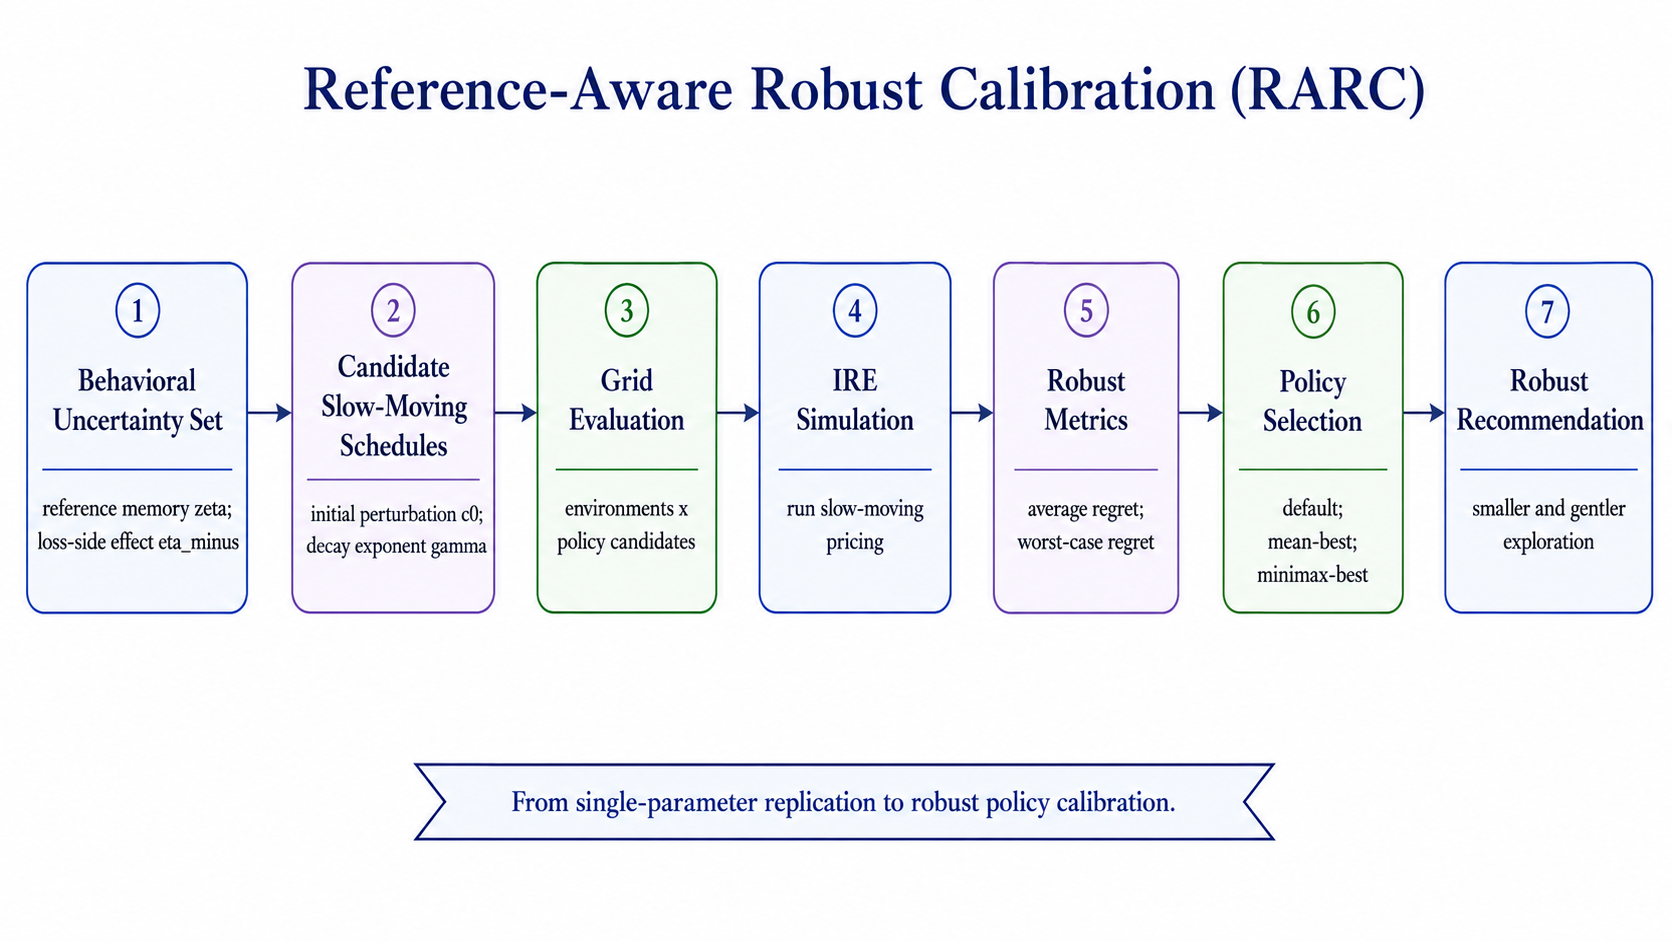
\includegraphics[width=0.92\textwidth]{rarc.png}
  \caption{RARC 流程。该扩展将 slow-moving schedule 选择转化为行为参数不确定下的稳健校准问题。}
  \label{fig:rarcworkflow}
\end{figure*}

\subsection{RARC 结果}
Table~\ref{tab:rarc} 展示 RARC 主要结果。默认候选依然表现稳健，平均最终 regret 为 $13.09$，最坏情形最终 regret 为 $14.39$。但在本不确定集下，平均表现和 minimax 稳健表现最好的候选都是 $(c_0,\gamma)=(0.05,0.20)$，平均最终 regret 为 $10.62$，最坏情形最终 regret 为 $13.32$。较大的初始扰动 $c_0=0.15$ 表现明显更差，特别是在高参考记忆与强损失侧效应环境中风险更高。

\begin{table*}[t]
\centering
\caption{RARC 在九个不确定环境下的候选策略汇总。}
\label{tab:rarc}
\begin{tabular}{lrrrrl}
\hline
候选 & $c_0$ & 衰减指数 & 平均最终 regret & 最坏情形最终 regret & 角色\\
\hline
c0\_0\_05\_decay\_0\_20 & 0.05 & 0.20 & 10.62 & 13.32 & mean-best; minimax-best\\
c0\_0\_05\_decay\_0\_25 & 0.05 & 0.25 & 10.70 & 13.78 & candidate\\
c0\_0\_05\_decay\_0\_30 & 0.05 & 0.30 & 10.82 & 14.19 & candidate\\
c0\_0\_10\_decay\_0\_25 & 0.10 & 0.25 & 13.09 & 14.39 & default\\
c0\_0\_15\_decay\_0\_30 & 0.15 & 0.30 & 17.12 & 24.35 & high-risk candidate\\
\hline
\end{tabular}
\end{table*}

Table~\ref{tab:environment} 展示了 RARC 的环境压力模式。最容易的环境是参考记忆较短且损失侧参考效应较弱的组合；最困难的环境是 $\zeta=0.40$ 且 $\eta^-=0.45$，平均候选 regret 达到 $17.06$，最差候选达到 $24.35$。这与模型机制一致：参考价格越持久、损失惩罚越强，状态污染的长期代价越高。

\begin{table*}[t]
\centering
\caption{RARC 在各不确定环境下的聚合结果。}
\label{tab:environment}
\begin{tabular}{rrrrr}
\hline
$\zeta$ & $\eta^-$ & 平均最终 regret & 最优最终 regret & 最差最终 regret\\
\hline
0.02 & 0.15 & 12.18 & 9.44 & 15.44\\
0.02 & 0.30 & 12.65 & 9.76 & 16.73\\
0.02 & 0.45 & 13.71 & 10.63 & 17.22\\
0.10 & 0.15 & 12.34 & 9.51 & 15.64\\
0.10 & 0.30 & 12.96 & 9.90 & 17.04\\
0.10 & 0.45 & 13.99 & 10.96 & 17.72\\
0.40 & 0.15 & 13.41 & 10.37 & 16.79\\
0.40 & 0.30 & 15.14 & 11.40 & 20.80\\
0.40 & 0.45 & 17.06 & 13.32 & 24.35\\
\hline
\end{tabular}
\end{table*}

Figure~\ref{fig:rarc} 对该结论进行可视化。热力图显示，在本不确定集下较小扰动整体优于较大扰动；前沿图显示 mean-best 与 minimax-best 重合，说明该稳健候选并非只保护单一极端场景，而是在平均表现和最坏情形之间同时占优。

\begin{figure*}[t]
  \centering
  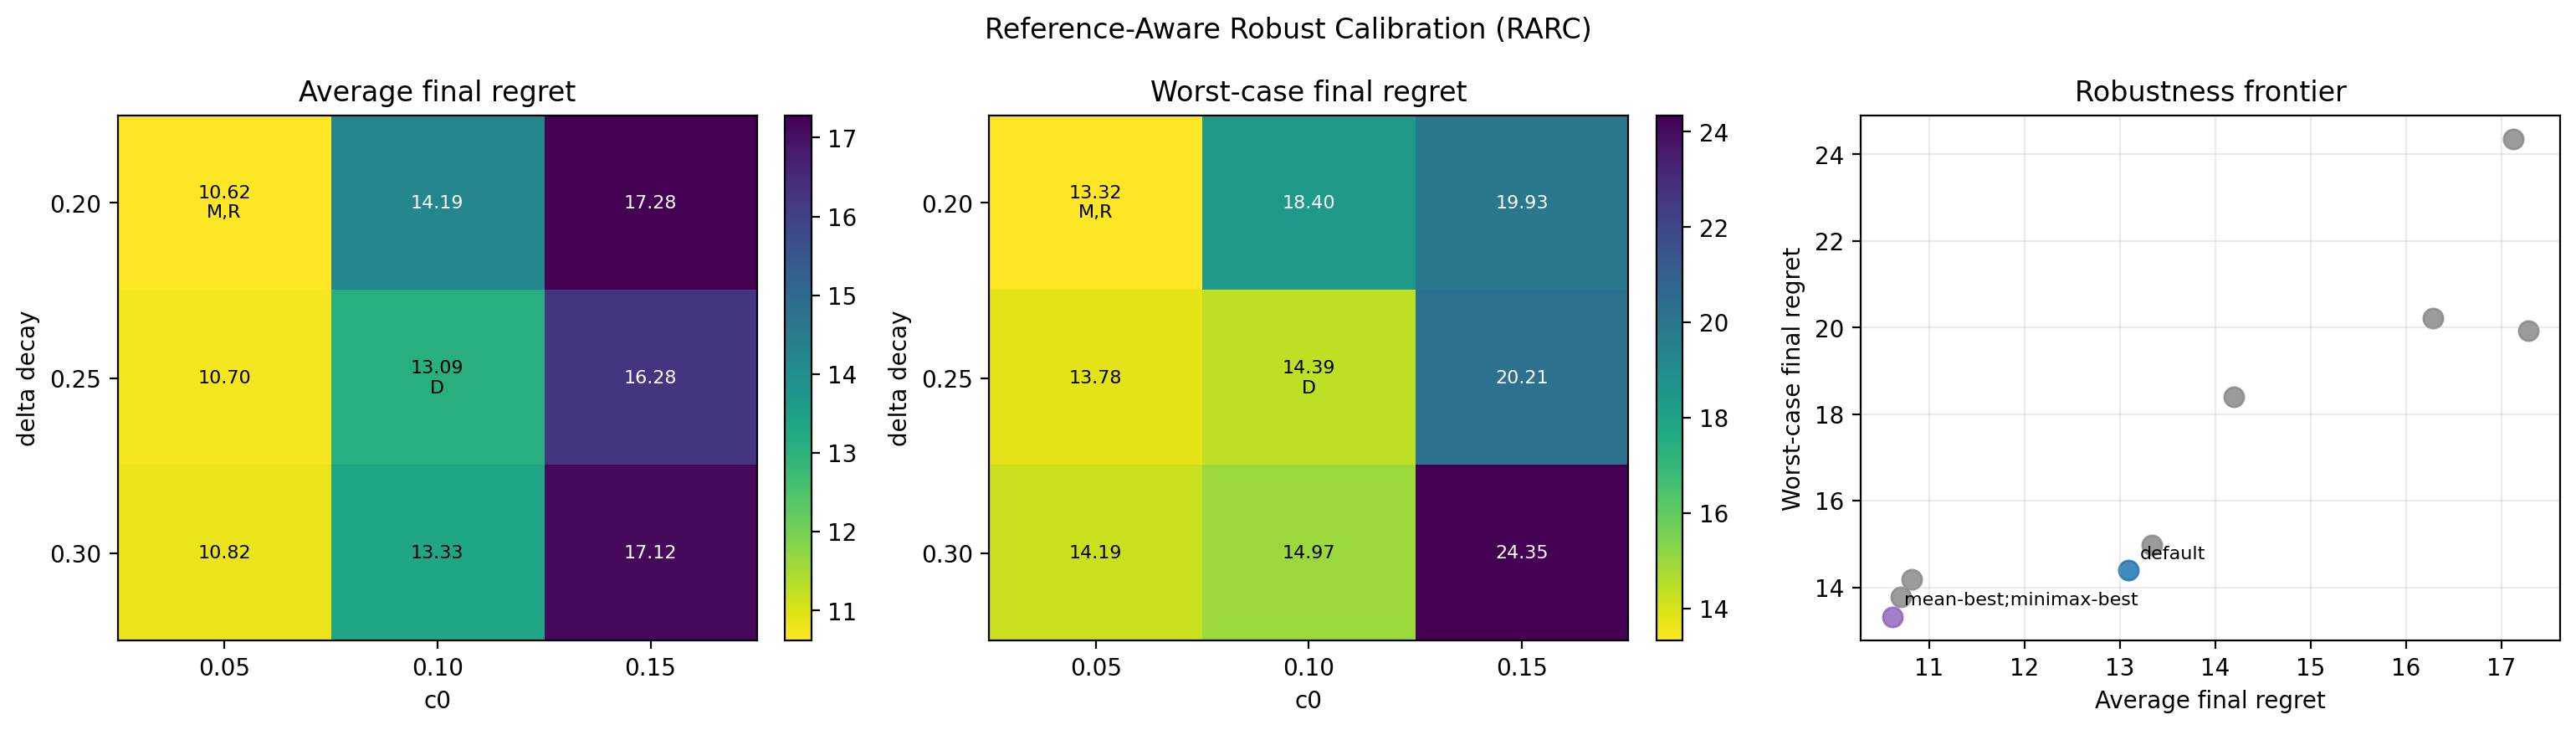
\includegraphics[width=0.96\textwidth]{robust_calibration.png}
  \caption{RARC 扩展实验。热力图比较平均最终 regret 与最坏情形最终 regret；前沿图比较平均表现与稳健表现。}
  \label{fig:rarc}
\end{figure*}

RARC 的运筹学解释是：slow-moving 的结构思想是正确的，但参数校准仍然重要。如果初始扰动过大，策略会产生不必要的收入损失和更大的参考状态扰动；如果在大扰动后过快衰减，早期状态损伤仍可能影响后续收益。本实验中更小初始扰动配合更慢衰减更稳健，这与论文机制一致：探索应足够局部，以降低参考状态污染。

\subsection{RARC 的新增价值}
RARC 增加了一层主复现实验中没有显式讨论的设计问题。复现实验回答的是：在一组参数下，slow-moving 结构是否有效；RARC 回答的是：当行为环境发生变化时，slow-moving 的 schedule 是否稳定。这更接近实际企业面对的问题，因为企业通常无法在实验前准确知道消费者参考价格记忆和损失厌恶强度。

RARC 还帮助解释探索幅度的作用。更大的价格扰动不一定更好，因为它同时带来两种代价：一是当期收入损失，二是参考价格状态变化。本实验中最优候选使用较小初始扰动，说明在这些环境下，额外价格离散度带来的统计收益低于状态控制成本。

最后，RARC 为后续算法扩展提供了入口。更完整的自适应策略可以从保守扰动开始，并根据对需求和参考记忆的学习结果调整 $c_0$ 和衰减速度。当前 RARC 没有实现这一闭环，但它明确了哪些设计变量重要，并通过数值结果证明这些变量确实影响 regret。

\section{运筹学视角讨论}
\subsection{稳健优化视角}
RARC 可以被理解为一个小型稳健优化问题。决策变量是 slow-moving schedule 中的 $c_0$ 和 $\gamma$；不确定集是行为参数 $\zeta$ 和 $\eta^-$ 的可能取值；目标不仅是在平均环境中表现好，也要避免在最困难环境中表现过差。这与运筹学中的稳健决策思想一致：很多管理决策必须在参数尚未完全确定时提前做出。

minimax 视角改变了我们评价 slow-moving policy 的方式。一个 schedule 在单一校准环境中表现好，并不代表它在参考价格更持久或损失厌恶更强时仍然安全。相反，稍微保守的 schedule 如果能显著降低下行风险，就具有管理价值。在本实验网格中，同一候选同时最小化平均最终 regret 和最坏情形最终 regret，因此参数建议比较清晰。

\subsection{在线学习视角}
论文也揭示了在线学习中的一个重要事实：由策略生成的数据并不总是被动观测。在很多运营系统中，行动会改变未来状态，并进一步改变后续观测的分布。这会形成学习与控制之间的反馈。deterministic testing 失败，是因为它忽略了这种反馈；slow-moving 成功，是因为它控制了反馈通道。

这一点可以推广到库存实验、平台排序、促销计划等问题。在这些问题中，实验行为可能改变客户行为、库存位置或未来需求构成。因此，策略不能只根据短期估计精度来评价，而应根据长期系统响应来评价。Regret 框架的价值就在于，它把这种累计影响纳入统一指标。

\subsection{管理视角}
对管理者而言，核心启发是：当消费者会记住价格时，价格实验应当更渐进。大幅折扣可能带来短期销量和需求信息，但也可能把参考价格拉低；突然涨价可能帮助识别需求弹性，但也可能制造强烈损失感。slow-moving policy 提供了一个替代方案：围绕当前估计价格做局部测试，让市场状态逐渐稳定，再根据足够观测更新价格。

RARC 进一步给出不确定市场中的操作建议。如果企业不确定消费者记忆强度和损失厌恶程度，那么从较小扰动开始通常比激进测试更安全。这并不意味着取消探索，而是要求探索强度同时考虑统计信息价值和行为状态成本。

\section{优势、局限与未来扩展}
\subsection{方法优势}
该方法的主要优势是概念清晰。它指出普通学习策略失败的根源：价格实验不是状态中性的，历史价格会塑造未来需求状态。slow-moving pricing 也具有很强的可解释性，不依赖复杂黑箱优化，而是使用 episode、双侧扰动和普通最小二乘。

数值证据也较有说服力。Figure~\ref{fig:figure2} 和 Figure~\ref{fig:figure5} 构成直接对照：忽略参考效应会导致 regret 大幅上升，而显式控制参考价格状态可以抑制这种上升。RARC 扩展进一步说明，slow-moving 的扰动计划可以被视为可校准的稳健设计对象。

\subsection{局限性}
局限同样明显。第一，实验基于合成线性需求模型，真实需求可能非线性、受库存截断、受竞争价格影响，或受到季节性和用户分层等协变量驱动。第二，仿真路径数较少，因此不能过度解读最终数值的细微差异。第三，slow-moving policy 主要针对 loss-averse 的时变参考价格环境；若消费者行为变成 gain-seeking，最优策略结构可能不同。第四，RARC 是数值扩展，能够给出稳健参数选择建议，但并未证明所选候选具有新的 regret 上界。

\subsection{可能扩展}
理论扩展可以放宽参考价格过程假设。例如，可以研究异质记忆率、参考价格随机跳变或部分可观测的参考状态分布。核心问题是：当状态过程更持久、更难预测时，是否仍能保持 $O(\sqrt{T})$ regret。

算法扩展可以将 slow-moving pricing 与置信区间、贝叶斯学习或 bandit 方法结合。扰动幅度不一定固定衰减，而可以根据估计不确定性和状态污染风险自适应调整。RARC 是这一方向的第一步，因为它把 schedule 选择明确建模为稳健校准问题。

应用扩展包括零售促销日历、订阅续费定价、平台价格实验和高频折扣品类。实际企业不应只用短期销量评价价格实验，还应评估实验如何改变未来消费者预期。这要求把定价实验与搜索行为、复购历史、加购行为和折扣响应等行为数据结合。

\subsection{论文其他方向对本项目的启发}
除时变参考价格外，论文还讨论了 fixed reference price 场景。在该场景中，参考价格不随历史价格变化，但收入函数在参考价附近存在 kink。卖家如果只在 kink 的一侧采样，就无法学习另一侧需求斜率，容易出现 incomplete learning。因此，一个自然后续实验是实现 quick learning policy，强制在参考价两侧采样，并与被动 certainty-equivalence 策略对比。

另一个值得延伸的方向是 gain-seeking 行为。当消费者对“价格低于参考价”的获得感反应更强时，最优价格路径可能不再是稳定价格附近的慢变化，而可能呈现循环降价或 price skimming 结构。这说明参考价格效应不只是改变参数估计，还可能改变最优控制结构。若后续扩展这一部分，应先确定最优循环长度，再讨论未知参数下如何学习该循环。

论文还提出过用于识别 loss-aversion 与 gain-seeking 的统计检验思路。该方向对应用很重要，因为企业在选择 slow-moving 或循环定价策略之前，需要先判断消费者行为类型。将统计检验、RARC 稳健校准和后续定价策略连接起来，可以形成一个更完整的应用流程：先识别行为机制，再选择策略结构，最后根据不确定性校准扰动参数。

\begin{table}[H]
\centering
\scriptsize
\setlength{\tabcolsep}{1pt}
\caption{未来扩展路线图。}
\label{tab:roadmap}
\begin{tabular}{p{0.12\columnwidth}p{0.31\columnwidth}p{0.25\columnwidth}p{0.22\columnwidth}}
\hline
方向 & 研究问题 & 可能方法 & 预期贡献\\
\hline
理论 & 更一般参考价过程下能否保持 regret 保证 & 一般状态偏差界 & 扩展 $O(\sqrt{T})$ 条件\\
理论 & 消费者异质性如何改变学习 & 潜在状态或混合模型 & 分群参考价格控制\\
算法 & 扰动能否在线自适应 & 置信区间或贝叶斯更新 & 状态感知自适应探索\\
算法 & RARC 能否序贯化 & minimax 或分布稳健校准 & 不依赖固定网格的稳健 schedule\\
应用 & 促销日历如何设计 & 加入日历约束和参考状态 & 减少长期促销伤害\\
应用 & 企业如何测量参考效应 & 交易数据结合行为信号 & 支持落地的参考状态估计\\
\hline
\end{tabular}
\end{table}

\section{结论}
本项目复现并扩展了 den Boer 与 Keskin 的核心数值结论 \cite{denBoerKeskin2022}。带参考价格效应的动态定价与普通需求学习有本质区别，因为卖家的价格行为会创造影响未来需求的状态。deterministic testing 在无参考效应时表现良好，但在 reference-effect 场景下出现明显模型失配。slow-moving pricing 的优势在于同时设计探索和状态控制。

新增 RARC 实验给出进一步的实际启发：在测试的不确定环境中，默认 slow-moving 参数已经较稳健，但较小初始扰动和较慢衰减能够获得更低的平均最终 regret 与最坏情形 regret。这支持了论文背后的更一般运筹学原则：在具有内生行为状态的动态系统中，好的学习算法不仅要统计效率高，还要谨慎管理自身行动对系统状态的改变。

\bibliographystyle{IEEEtran}
\bibliography{../bib/references}

\end{document}
